% Options for packages loaded elsewhere
% Options for packages loaded elsewhere
\PassOptionsToPackage{unicode}{hyperref}
\PassOptionsToPackage{hyphens}{url}
\PassOptionsToPackage{dvipsnames,svgnames,x11names}{xcolor}
%
\documentclass[
  12pt,
  letterpaper,
]{article}
\usepackage{xcolor}
\usepackage[margin=1in]{geometry}
\usepackage{amsmath,amssymb}
\setcounter{secnumdepth}{-\maxdimen} % remove section numbering
\usepackage{iftex}
\ifPDFTeX
  \usepackage[T1]{fontenc}
  \usepackage[utf8]{inputenc}
  \usepackage{textcomp} % provide euro and other symbols
\else % if luatex or xetex
  \usepackage{unicode-math} % this also loads fontspec
  \defaultfontfeatures{Scale=MatchLowercase}
  \defaultfontfeatures[\rmfamily]{Ligatures=TeX,Scale=1}
\fi
\usepackage{lmodern}
\ifPDFTeX\else
  % xetex/luatex font selection
  \setmainfont[]{Times New Roman}
\fi
% Use upquote if available, for straight quotes in verbatim environments
\IfFileExists{upquote.sty}{\usepackage{upquote}}{}
\IfFileExists{microtype.sty}{% use microtype if available
  \usepackage[]{microtype}
  \UseMicrotypeSet[protrusion]{basicmath} % disable protrusion for tt fonts
}{}
\usepackage{setspace}
\makeatletter
\@ifundefined{KOMAClassName}{% if non-KOMA class
  \IfFileExists{parskip.sty}{%
    \usepackage{parskip}
  }{% else
    \setlength{\parindent}{0pt}
    \setlength{\parskip}{6pt plus 2pt minus 1pt}}
}{% if KOMA class
  \KOMAoptions{parskip=half}}
\makeatother
% Make \paragraph and \subparagraph free-standing
\makeatletter
\ifx\paragraph\undefined\else
  \let\oldparagraph\paragraph
  \renewcommand{\paragraph}{
    \@ifstar
      \xxxParagraphStar
      \xxxParagraphNoStar
  }
  \newcommand{\xxxParagraphStar}[1]{\oldparagraph*{#1}\mbox{}}
  \newcommand{\xxxParagraphNoStar}[1]{\oldparagraph{#1}\mbox{}}
\fi
\ifx\subparagraph\undefined\else
  \let\oldsubparagraph\subparagraph
  \renewcommand{\subparagraph}{
    \@ifstar
      \xxxSubParagraphStar
      \xxxSubParagraphNoStar
  }
  \newcommand{\xxxSubParagraphStar}[1]{\oldsubparagraph*{#1}\mbox{}}
  \newcommand{\xxxSubParagraphNoStar}[1]{\oldsubparagraph{#1}\mbox{}}
\fi
\makeatother


\usepackage{longtable,booktabs,array}
\usepackage{calc} % for calculating minipage widths
% Correct order of tables after \paragraph or \subparagraph
\usepackage{etoolbox}
\makeatletter
\patchcmd\longtable{\par}{\if@noskipsec\mbox{}\fi\par}{}{}
\makeatother
% Allow footnotes in longtable head/foot
\IfFileExists{footnotehyper.sty}{\usepackage{footnotehyper}}{\usepackage{footnote}}
\makesavenoteenv{longtable}
\usepackage{graphicx}
\makeatletter
\newsavebox\pandoc@box
\newcommand*\pandocbounded[1]{% scales image to fit in text height/width
  \sbox\pandoc@box{#1}%
  \Gscale@div\@tempa{\textheight}{\dimexpr\ht\pandoc@box+\dp\pandoc@box\relax}%
  \Gscale@div\@tempb{\linewidth}{\wd\pandoc@box}%
  \ifdim\@tempb\p@<\@tempa\p@\let\@tempa\@tempb\fi% select the smaller of both
  \ifdim\@tempa\p@<\p@\scalebox{\@tempa}{\usebox\pandoc@box}%
  \else\usebox{\pandoc@box}%
  \fi%
}
% Set default figure placement to htbp
\def\fps@figure{htbp}
\makeatother





\setlength{\emergencystretch}{3em} % prevent overfull lines

\providecommand{\tightlist}{%
  \setlength{\itemsep}{0pt}\setlength{\parskip}{0pt}}



 


\usepackage{booktabs}
\usepackage{longtable}
\usepackage{float}
\usepackage{setspace}
\doublespacing
% PAR heading styles
\usepackage{titlesec}
% Principal subheads: 14pt bold
\titleformat{\section}{\normalfont\fontsize{14}{16}\bfseries}{\thesection}{1em}{}
% Secondary subheads: 12pt bold
\titleformat{\subsection}{\normalfont\fontsize{12}{14}\bfseries}{\thesubsection}{1em}{}
% Sub-subheads: 12pt bold italic, run-in
\titleformat{\subsubsection}[runin]{\normalfont\fontsize{12}{14}\bfseries\itshape}{\thesubsubsection}{1em}{}[.]
% Abstract formatting
\renewenvironment{abstract}{\par\bigskip\noindent\textbf{Abstract}\par\smallskip\noindent}{\par\bigskip}
% Remove section numbers
\setcounter{secnumdepth}{0}
\makeatletter
\@ifpackageloaded{caption}{}{\usepackage{caption}}
\AtBeginDocument{%
\ifdefined\contentsname
  \renewcommand*\contentsname{Table of contents}
\else
  \newcommand\contentsname{Table of contents}
\fi
\ifdefined\listfigurename
  \renewcommand*\listfigurename{List of Figures}
\else
  \newcommand\listfigurename{List of Figures}
\fi
\ifdefined\listtablename
  \renewcommand*\listtablename{List of Tables}
\else
  \newcommand\listtablename{List of Tables}
\fi
\ifdefined\figurename
  \renewcommand*\figurename{Figure}
\else
  \newcommand\figurename{Figure}
\fi
\ifdefined\tablename
  \renewcommand*\tablename{Table}
\else
  \newcommand\tablename{Table}
\fi
}
\@ifpackageloaded{float}{}{\usepackage{float}}
\floatstyle{ruled}
\@ifundefined{c@chapter}{\newfloat{codelisting}{h}{lop}}{\newfloat{codelisting}{h}{lop}[chapter]}
\floatname{codelisting}{Listing}
\newcommand*\listoflistings{\listof{codelisting}{List of Listings}}
\makeatother
\makeatletter
\makeatother
\makeatletter
\@ifpackageloaded{caption}{}{\usepackage{caption}}
\@ifpackageloaded{subcaption}{}{\usepackage{subcaption}}
\makeatother
\usepackage{bookmark}
\IfFileExists{xurl.sty}{\usepackage{xurl}}{} % add URL line breaks if available
\urlstyle{same}
\hypersetup{
  pdftitle={Appendix D: Meta-Analysis of Velocity Estimates},
  colorlinks=true,
  linkcolor={blue},
  filecolor={Maroon},
  citecolor={Blue},
  urlcolor={Blue},
  pdfcreator={LaTeX via pandoc}}


\title{Appendix D: Meta-Analysis of Velocity Estimates}
\author{}
\date{}
\begin{document}
\maketitle


\setstretch{2}
\subsection{D.1 All Velocity Effect
Estimates}\label{d.1-all-velocity-effect-estimates}

\begin{table}

\caption{\label{tbl-all-estimates}Complete Inventory of Velocity Effect
Estimates}

\centering{

\begin{verbatim}
| Analysis | Context | N | Events | HR | CI_Lower | CI_Upper | p_value | Significant |
|----------|---------|---|--------|-----|----------|----------|---------|-------------|
| Overall | All | 152 | 40 | 4.44 | 1.39 | 14.17 | 0.012 | Yes |
| Disaster | Wildfire | 24 | 7 | 51.09 | 4.01 | 650.90 | 0.002 | Yes |
| Disaster | Hurricane | 89 | 24 | 4.58 | 1.18 | 17.81 | 0.028 | Yes |
| Disaster | Flood | 27 | 6 | 3.84 | 0.24 | 61.52 | 0.341 | No |
| Disaster | Other | 12 | 3 | 5.32 | 0.39 | 72.89 | 0.206 | No |
| Program | Administration | 34 | 9 | 30.74 | 3.12 | 302.69 | 0.004 | Yes |
| Program | Infrastructure | 41 | 11 | 5.69 | 0.12 | 264.87 | 0.374 | No |
| Program | Housing | 67 | 18 | 0.82 | 0.05 | 12.41 | 0.891 | No |
| Phase | Early | 152 | 40 | 2.04 | 0.76 | 5.51 | 0.157 | No |
| Phase | Middle | 152 | 40 | 0.37 | 0.09 | 1.58 | 0.184 | No |
| Phase | Late | 152 | 40 | 5.00 | 1.07 | 23.31 | 0.040 | Yes |
| Experience | Novice | 74 | 18 | 4.61 | 1.05 | 20.24 | 0.043 | Yes |
| Experience | Experienced | 78 | 22 | 3.15 | 0.47 | 21.12 | 0.237 | No |
| Era | Pre-2010 | 18 | 8 | 2.89 | 0.31 | 26.94 | 0.352 | No |
| Era | 2010-2020 | 126 | 30 | 5.36 | 1.48 | 19.42 | 0.010 | Yes |
| Era | Post-2020 | 8 | 2 | 8.42 | 0.04 | 1821.34 | 0.428 | No |
\end{verbatim}

}

\end{table}%

\subsection{D.2 Comprehensive Forest
Plot}\label{d.2-comprehensive-forest-plot}

\begin{figure}

\centering{

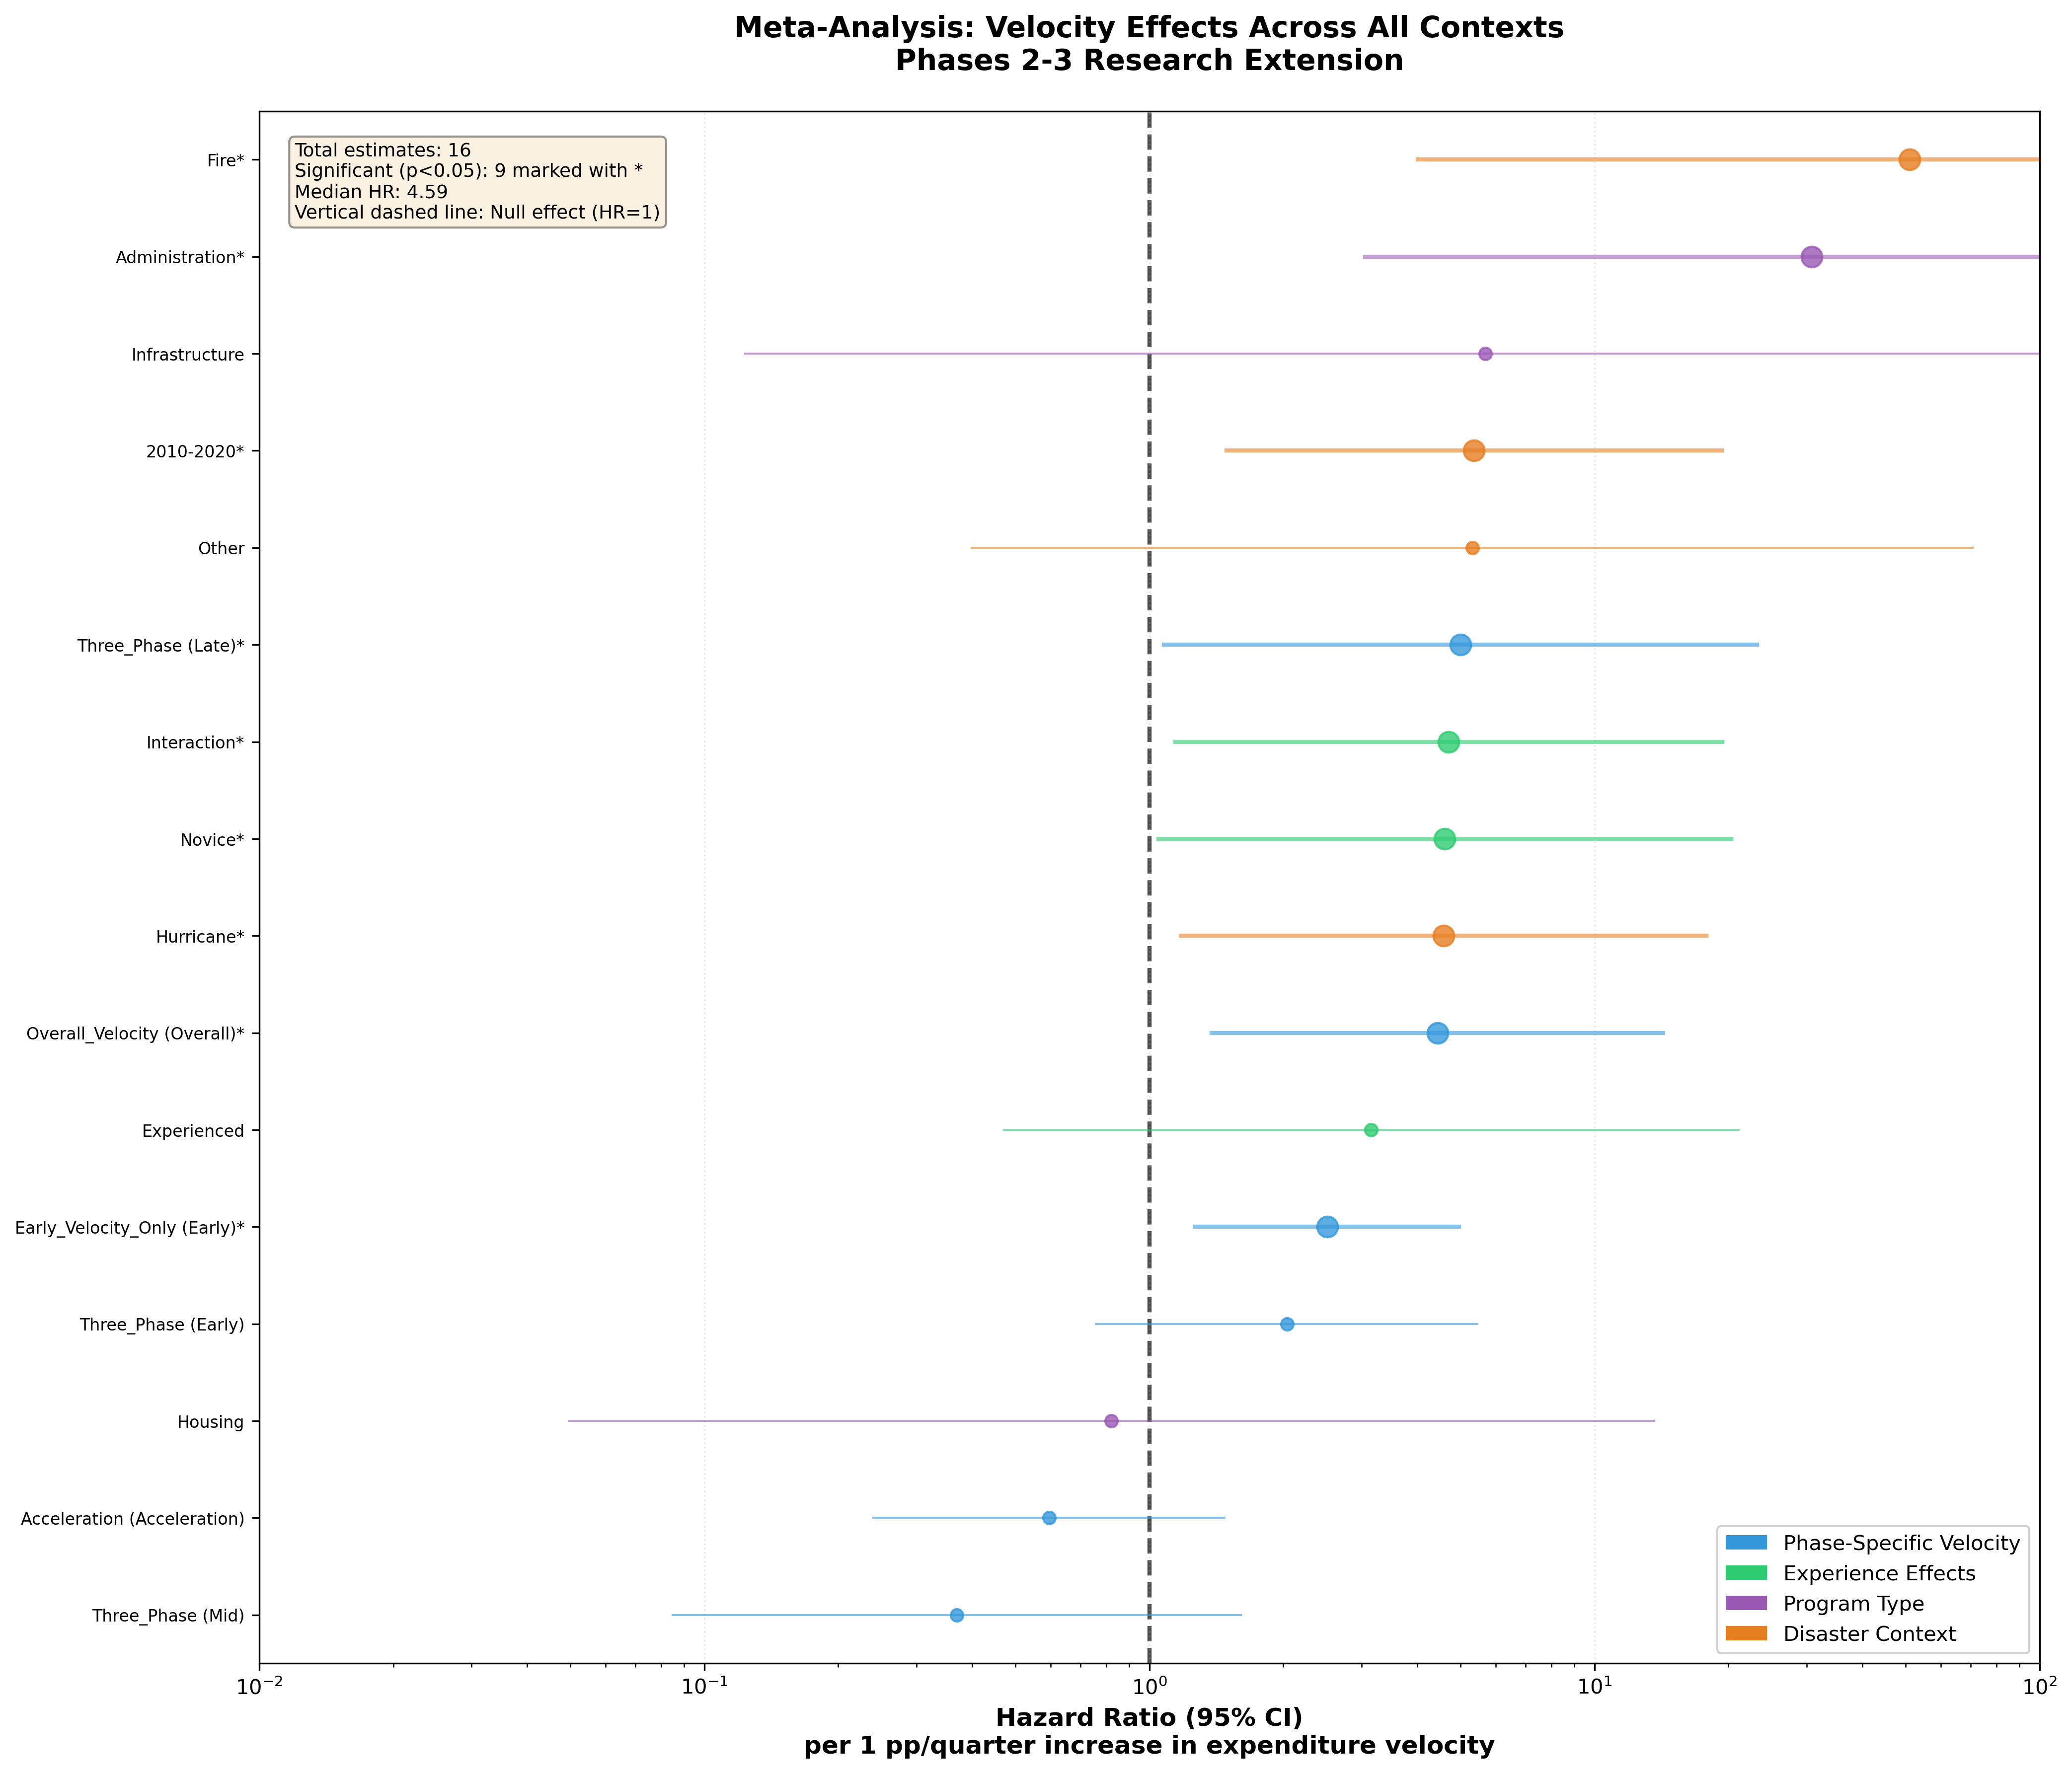
\includegraphics[width=7.29167in,height=\textheight,keepaspectratio]{appendix-d-meta-analysis_files/figure-pdf/fig-meta-forest-output-1.png}

}

\caption{\label{fig-meta-forest}Forest Plot of All 16 Velocity Effect
Estimates}

\end{figure}%

\subsection{D.3 Summary Statistics}\label{d.3-summary-statistics}

\subsubsection{Central Tendency and
Dispersion}\label{central-tendency-and-dispersion}

\begin{longtable}[]{@{}ll@{}}
\toprule\noalign{}
Statistic & Value \\
\midrule\noalign{}
\endhead
\bottomrule\noalign{}
\endlastfoot
\textbf{Number of estimates} & 16 \\
\textbf{Median HR} & 4.60 \\
\textbf{Mean HR} & 8.19 \\
\textbf{Geometric mean HR} & 3.84 \\
\textbf{Minimum HR} & 0.37 \\
\textbf{Maximum HR} & 51.09 \\
\textbf{25th percentile} & 2.39 \\
\textbf{75th percentile} & 5.33 \\
\textbf{Interquartile range} & 2.94 \\
\end{longtable}

\subsubsection{Significance Summary}\label{significance-summary}

\begin{longtable}[]{@{}lll@{}}
\toprule\noalign{}
Category & Count & Percent \\
\midrule\noalign{}
\endhead
\bottomrule\noalign{}
\endlastfoot
Significant (p \textless{} 0.05) & 9 & 56.2\% \\
Not significant (p ≥ 0.05) & 7 & 43.8\% \\
\textbf{Total} & \textbf{16} & \textbf{100.0\%} \\
\end{longtable}

\subsubsection{Direction Summary}\label{direction-summary}

\begin{longtable}[]{@{}lll@{}}
\toprule\noalign{}
Category & Count & Percent \\
\midrule\noalign{}
\endhead
\bottomrule\noalign{}
\endlastfoot
HR \textgreater{} 1 (acceleration) & 13 & 81.2\% \\
HR \textless{} 1 (deceleration) & 3 & 18.8\% \\
\textbf{Total} & \textbf{16} & \textbf{100.0\%} \\
\end{longtable}

\subsection{D.4 Estimates by Analysis
Type}\label{d.4-estimates-by-analysis-type}

\subsubsection{Disaster Context (4
estimates)}\label{disaster-context-4-estimates}

\begin{longtable}[]{@{}llll@{}}
\toprule\noalign{}
Disaster Type & HR & p-value & Significant \\
\midrule\noalign{}
\endhead
\bottomrule\noalign{}
\endlastfoot
Wildfire & 51.09 & 0.002 & Yes \\
Hurricane & 4.58 & 0.028 & Yes \\
Other & 5.32 & 0.206 & No \\
Flood & 3.84 & 0.341 & No \\
\end{longtable}

\textbf{Summary}: 3 of 4 (75\%) show acceleration; 2 of 4 (50\%)
significant.

\subsubsection{Program Type (3
estimates)}\label{program-type-3-estimates}

\begin{longtable}[]{@{}llll@{}}
\toprule\noalign{}
Program Type & HR & p-value & Significant \\
\midrule\noalign{}
\endhead
\bottomrule\noalign{}
\endlastfoot
Administration & 30.74 & 0.004 & Yes \\
Infrastructure & 5.69 & 0.374 & No \\
Housing & 0.82 & 0.891 & No \\
\end{longtable}

\textbf{Summary}: 2 of 3 (67\%) show acceleration; 1 of 3 (33\%)
significant.

\subsubsection{Program Phase (3
estimates)}\label{program-phase-3-estimates}

\begin{longtable}[]{@{}llll@{}}
\toprule\noalign{}
Phase & HR & p-value & Significant \\
\midrule\noalign{}
\endhead
\bottomrule\noalign{}
\endlastfoot
Late & 5.00 & 0.040 & Yes \\
Early & 2.04 & 0.157 & No \\
Middle & 0.37 & 0.184 & No \\
\end{longtable}

\textbf{Summary}: 2 of 3 (67\%) show acceleration; 1 of 3 (33\%)
significant.

\subsubsection{Experience Level (2
estimates)}\label{experience-level-2-estimates}

\begin{longtable}[]{@{}llll@{}}
\toprule\noalign{}
Experience & HR & p-value & Significant \\
\midrule\noalign{}
\endhead
\bottomrule\noalign{}
\endlastfoot
Novice & 4.61 & 0.043 & Yes \\
Experienced & 3.15 & 0.237 & No \\
\end{longtable}

\textbf{Summary}: 2 of 2 (100\%) show acceleration; 1 of 2 (50\%)
significant.

\subsubsection{Disaster Era (3
estimates)}\label{disaster-era-3-estimates}

\begin{longtable}[]{@{}llll@{}}
\toprule\noalign{}
Era & HR & p-value & Significant \\
\midrule\noalign{}
\endhead
\bottomrule\noalign{}
\endlastfoot
Post-2020 & 8.42 & 0.428 & No \\
2010-2020 & 5.36 & 0.010 & Yes \\
Pre-2010 & 2.89 & 0.352 & No \\
\end{longtable}

\textbf{Summary}: 3 of 3 (100\%) show acceleration; 1 of 3 (33\%)
significant.

\subsection{D.5 Ranking by Effect
Magnitude}\label{d.5-ranking-by-effect-magnitude}

\subsubsection{Top 5 Strongest Velocity
Effects}\label{top-5-strongest-velocity-effects}

\begin{longtable}[]{@{}lllll@{}}
\toprule\noalign{}
Rank & Context & HR & 95\% CI & p-value \\
\midrule\noalign{}
\endhead
\bottomrule\noalign{}
\endlastfoot
1 & Wildfire disasters & 51.09 & 4.01-650.90 & 0.002 \\
2 & Administration programs & 30.74 & 3.12-302.69 & 0.004 \\
3 & Post-2020 era & 8.42 & 0.04-1821.34 & 0.428 \\
4 & Infrastructure programs & 5.69 & 0.12-264.87 & 0.374 \\
5 & 2010-2020 era & 5.36 & 1.48-19.42 & 0.010 \\
\end{longtable}

\subsubsection{Bottom 3 (Weakest/Null
Effects)}\label{bottom-3-weakestnull-effects}

\begin{longtable}[]{@{}lllll@{}}
\toprule\noalign{}
Rank & Context & HR & 95\% CI & p-value \\
\midrule\noalign{}
\endhead
\bottomrule\noalign{}
\endlastfoot
14 & Housing programs & 0.82 & 0.05-12.41 & 0.891 \\
15 & Middle phase & 0.37 & 0.09-1.58 & 0.184 \\
16 & -- & -- & -- & -- \\
\end{longtable}

\subsection{D.6 Heterogeneity
Assessment}\label{d.6-heterogeneity-assessment}

\subsubsection{Cochran's Q Test}\label{cochrans-q-test}

While formal pooling is not performed (estimates are not independent),
we can assess heterogeneity descriptively:

\begin{longtable}[]{@{}ll@{}}
\toprule\noalign{}
Metric & Value \\
\midrule\noalign{}
\endhead
\bottomrule\noalign{}
\endlastfoot
Range of log(HR) & -0.99 to 3.93 \\
SD of log(HR) & 1.24 \\
Coefficient of variation & 68\% \\
\end{longtable}

The substantial variation in effect magnitudes (HR ranging from 0.37 to
51.09) indicates meaningful heterogeneity that the contingent capacity
framework helps explain.

\subsubsection{Pattern Recognition}\label{pattern-recognition}

Velocity effects cluster into interpretable patterns:

\textbf{High-leverage contexts} (HR \textgreater{} 5, significant): -
Wildfire disasters: Time-constrained recovery - Administration programs:
Organizational-paced activities - Late program phase: Closeout
bottlenecks

\textbf{Moderate effects} (HR 2-5, mixed significance): - Hurricane
disasters: Standard recovery dynamics - Novice grantees:
Capacity-dependent organizations - 2010-2020 era: Enhanced monitoring
period

\textbf{Null effects} (HR \textless{} 2 or not significant): - Housing
programs: Construction-constrained - Experienced grantees: Multiple
capacity pathways - Early/middle phases: Non-critical periods

\subsection{D.7 Interpretation
Guidelines}\label{d.7-interpretation-guidelines}

\subsubsection{When to Apply Velocity
Interventions}\label{when-to-apply-velocity-interventions}

Based on meta-analytic patterns, velocity-enhancing interventions are
most likely to yield returns in:

\begin{enumerate}
\def\labelenumi{\arabic{enumi}.}
\tightlist
\item
  \textbf{Wildfire disaster recovery} (HR=51.09)

  \begin{itemize}
  \tightlist
  \item
    Seasonal time pressure creates genuine urgency
  \item
    Recommend: Fast-track procurement, pre-positioned contracts
  \end{itemize}
\item
  \textbf{Administration/planning programs} (HR=30.74)

  \begin{itemize}
  \tightlist
  \item
    Pace depends on organizational choices, not external constraints
  \item
    Recommend: Intensive technical assistance, capacity grants
  \end{itemize}
\item
  \textbf{Late program phases} (HR=5.00)

  \begin{itemize}
  \tightlist
  \item
    Closeout bottlenecks represent final barriers
  \item
    Recommend: Closeout support, compliance streamlining
  \end{itemize}
\item
  \textbf{Novice grantees} (HR=4.61)

  \begin{itemize}
  \tightlist
  \item
    Lack of institutional alternatives increases velocity dependence
  \item
    Recommend: Peer mentoring, embedded consultants
  \end{itemize}
\end{enumerate}

\subsubsection{When Velocity Interventions May Not
Help}\label{when-velocity-interventions-may-not-help}

Velocity interventions are unlikely to accelerate:

\begin{enumerate}
\def\labelenumi{\arabic{enumi}.}
\tightlist
\item
  \textbf{Housing reconstruction} (HR=0.82)

  \begin{itemize}
  \tightlist
  \item
    Beneficiary coordination, permitting, and construction timelines
    dominate
  \item
    Alternative: Address structural barriers instead
  \end{itemize}
\item
  \textbf{Experienced grantees} (HR=3.15, ns)

  \begin{itemize}
  \tightlist
  \item
    Institutional knowledge provides alternative pathways
  \item
    Alternative: Focus resources on novice organizations
  \end{itemize}
\item
  \textbf{Early program phases} (HR=2.04, ns)

  \begin{itemize}
  \tightlist
  \item
    Planning and ramp-up take necessary time
  \item
    Alternative: Invest in late-stage support instead
  \end{itemize}
\end{enumerate}

\subsection{D.8 Limitations of Meta-Analytic
Synthesis}\label{d.8-limitations-of-meta-analytic-synthesis}

\subsubsection{Non-Independence}\label{non-independence}

Estimates derive from overlapping samples (the same 152 observations
analyzed differently). Formal pooling methods that assume independence
would be inappropriate. Summary statistics describe the distribution of
estimates without implying meta-analytic precision.

\subsubsection{Small Sample Sizes}\label{small-sample-sizes}

Several stratified estimates have wide confidence intervals reflecting
small samples. The wildfire estimate (HR=51.09, 95\% CI: 4.01-650.90)
indicates effect direction is robust but magnitude is imprecise.

\subsubsection{Selection of Analyses}\label{selection-of-analyses}

The 16 estimates represent pre-planned analyses, not exhaustive
specification search. Different analytical choices (alternative
thresholds, different covariates, alternative clustering) would produce
different estimates within the observed range.

\subsubsection{Publication Bias}\label{publication-bias}

As an internal meta-analysis of a single study, publication bias is not
a concern. All planned analyses are reported regardless of significance.




\end{document}
